% Options for packages loaded elsewhere
\PassOptionsToPackage{unicode}{hyperref}
\PassOptionsToPackage{hyphens}{url}
%
\documentclass[
  ignorenonframetext,
]{beamer}
\usepackage{pgfpages}
\setbeamertemplate{caption}[numbered]
\setbeamertemplate{caption label separator}{: }
\setbeamercolor{caption name}{fg=normal text.fg}
\beamertemplatenavigationsymbolsempty
% Prevent slide breaks in the middle of a paragraph
\widowpenalties 1 10000
\raggedbottom
\setbeamertemplate{part page}{
  \centering
  \begin{beamercolorbox}[sep=16pt,center]{part title}
    \usebeamerfont{part title}\insertpart\par
  \end{beamercolorbox}
}
\setbeamertemplate{section page}{
  \centering
  \begin{beamercolorbox}[sep=12pt,center]{part title}
    \usebeamerfont{section title}\insertsection\par
  \end{beamercolorbox}
}
\setbeamertemplate{subsection page}{
  \centering
  \begin{beamercolorbox}[sep=8pt,center]{part title}
    \usebeamerfont{subsection title}\insertsubsection\par
  \end{beamercolorbox}
}
\AtBeginPart{
  \frame{\partpage}
}
\AtBeginSection{
  \ifbibliography
  \else
    \frame{\sectionpage}
  \fi
}
\AtBeginSubsection{
  \frame{\subsectionpage}
}

\usepackage{amsmath,amssymb}
\usepackage{iftex}
\ifPDFTeX
  \usepackage[T1]{fontenc}
  \usepackage[utf8]{inputenc}
  \usepackage{textcomp} % provide euro and other symbols
\else % if luatex or xetex
  \usepackage{unicode-math}
  \defaultfontfeatures{Scale=MatchLowercase}
  \defaultfontfeatures[\rmfamily]{Ligatures=TeX,Scale=1}
\fi
\usepackage{lmodern}
\usecolortheme{seagull}
\ifPDFTeX\else  
    % xetex/luatex font selection
\fi
% Use upquote if available, for straight quotes in verbatim environments
\IfFileExists{upquote.sty}{\usepackage{upquote}}{}
\IfFileExists{microtype.sty}{% use microtype if available
  \usepackage[]{microtype}
  \UseMicrotypeSet[protrusion]{basicmath} % disable protrusion for tt fonts
}{}
\makeatletter
\@ifundefined{KOMAClassName}{% if non-KOMA class
  \IfFileExists{parskip.sty}{%
    \usepackage{parskip}
  }{% else
    \setlength{\parindent}{0pt}
    \setlength{\parskip}{6pt plus 2pt minus 1pt}}
}{% if KOMA class
  \KOMAoptions{parskip=half}}
\makeatother
\usepackage{xcolor}
\newif\ifbibliography
\ifLuaTeX
  \usepackage{luacolor}
  \usepackage[soul]{lua-ul}
\else
  \usepackage{soul}
  \makeatletter
  \let\HL\hl
  \renewcommand\hl{% fix for beamer highlighting
    \let\set@color\beamerorig@set@color
    \let\reset@color\beamerorig@reset@color
    \HL}
  \makeatother
  
\fi
\setlength{\emergencystretch}{3em} % prevent overfull lines
\setcounter{secnumdepth}{-\maxdimen} % remove section numbering


\providecommand{\tightlist}{%
  \setlength{\itemsep}{0pt}\setlength{\parskip}{0pt}}\usepackage{longtable,booktabs,array}
\usepackage{calc} % for calculating minipage widths
\usepackage{caption}
% Make caption package work with longtable
\makeatletter
\def\fnum@table{\tablename~\thetable}
\makeatother
\usepackage{graphicx}
\makeatletter
\def\maxwidth{\ifdim\Gin@nat@width>\linewidth\linewidth\else\Gin@nat@width\fi}
\def\maxheight{\ifdim\Gin@nat@height>\textheight\textheight\else\Gin@nat@height\fi}
\makeatother
% Scale images if necessary, so that they will not overflow the page
% margins by default, and it is still possible to overwrite the defaults
% using explicit options in \includegraphics[width, height, ...]{}
\setkeys{Gin}{width=\maxwidth,height=\maxheight,keepaspectratio}
% Set default figure placement to htbp
\makeatletter
\def\fps@figure{htbp}
\makeatother

\makeatletter
\@ifpackageloaded{caption}{}{\usepackage{caption}}
\AtBeginDocument{%
\ifdefined\contentsname
  \renewcommand*\contentsname{Table of contents}
\else
  \newcommand\contentsname{Table of contents}
\fi
\ifdefined\listfigurename
  \renewcommand*\listfigurename{List of Figures}
\else
  \newcommand\listfigurename{List of Figures}
\fi
\ifdefined\listtablename
  \renewcommand*\listtablename{List of Tables}
\else
  \newcommand\listtablename{List of Tables}
\fi
\ifdefined\figurename
  \renewcommand*\figurename{Figure}
\else
  \newcommand\figurename{Figure}
\fi
\ifdefined\tablename
  \renewcommand*\tablename{Table}
\else
  \newcommand\tablename{Table}
\fi
}
\@ifpackageloaded{float}{}{\usepackage{float}}
\floatstyle{ruled}
\@ifundefined{c@chapter}{\newfloat{codelisting}{h}{lop}}{\newfloat{codelisting}{h}{lop}[chapter]}
\floatname{codelisting}{Listing}
\newcommand*\listoflistings{\listof{codelisting}{List of Listings}}
\makeatother
\makeatletter
\makeatother
\makeatletter
\@ifpackageloaded{caption}{}{\usepackage{caption}}
\@ifpackageloaded{subcaption}{}{\usepackage{subcaption}}
\makeatother

\ifLuaTeX
  \usepackage{selnolig}  % disable illegal ligatures
\fi
\usepackage{bookmark}

\IfFileExists{xurl.sty}{\usepackage{xurl}}{} % add URL line breaks if available
\urlstyle{same} % disable monospaced font for URLs
\hypersetup{
  pdftitle={How did Australians behave during the COVID-19 pandemic?},
  pdfauthor={Gerry Ryan; Nick Golding; August Hao; Katharine Senior; David Price; Oliver Eales; Mingmei Teo; James McCaw; Freya Shearer; AUTHORS FROM TEST SEEKING BEHAVIOURS PAPER},
  hidelinks,
  pdfcreator={LaTeX via pandoc}}


\title{How did Australians behave during the COVID-19 pandemic?}
\subtitle{A look into mobility and systematic questionnaire data from
2020-2023}
\author{Gerry Ryan \and Nick Golding \and August Hao \and Katharine
Senior \and David Price \and Oliver Eales \and Mingmei Teo \and James
McCaw \and Freya Shearer \and AUTHORS FROM TEST SEEKING BEHAVIOURS
PAPER}
\date{}

\begin{document}
\frame{\titlepage}


\begin{frame}{Remember a time}
\phantomsection\label{remember-a-time}
\begin{columns}[T]
\begin{column}{0.3\textwidth}
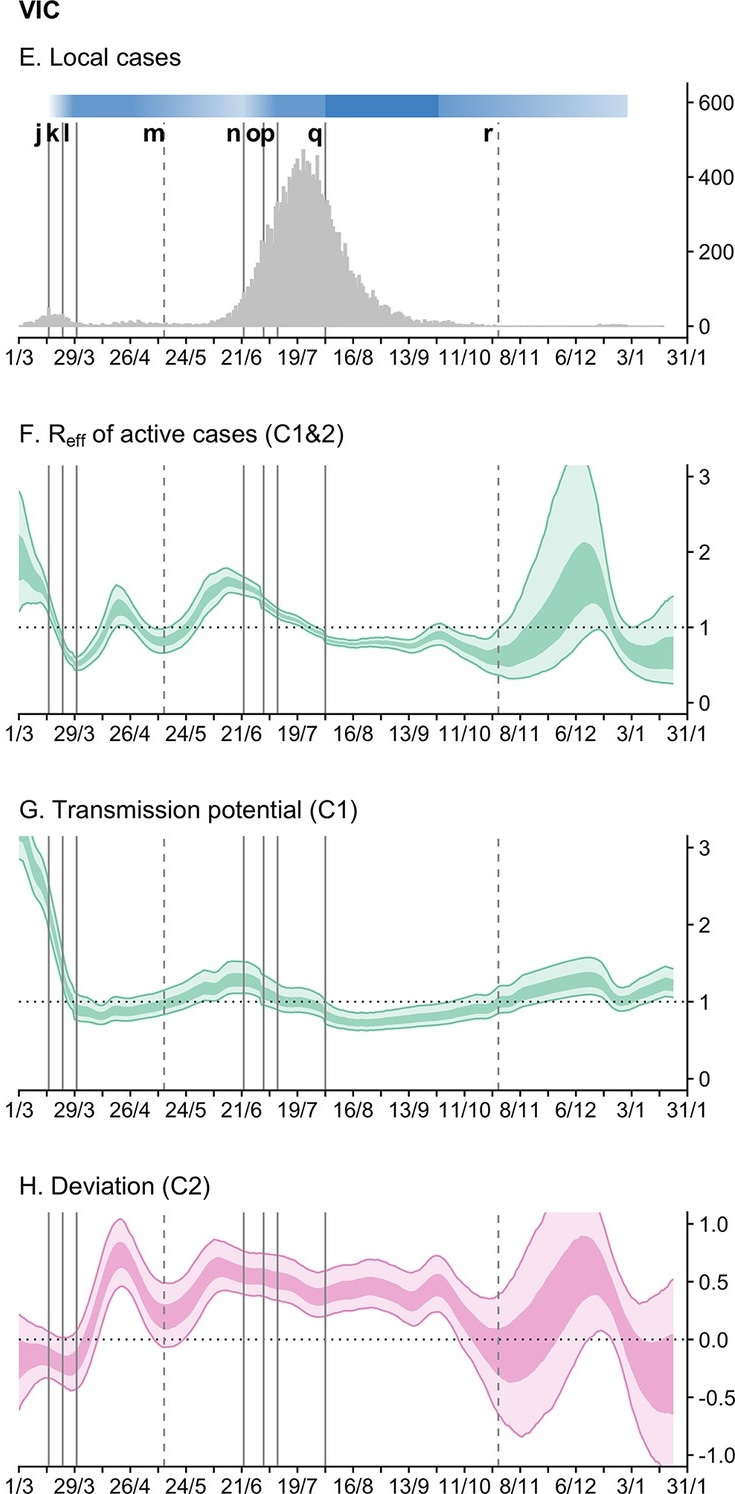
\includegraphics{images/lax_78089_elife-78089-fig2-v2.tif.jpg}
\end{column}

\begin{column}{0.3\textwidth}
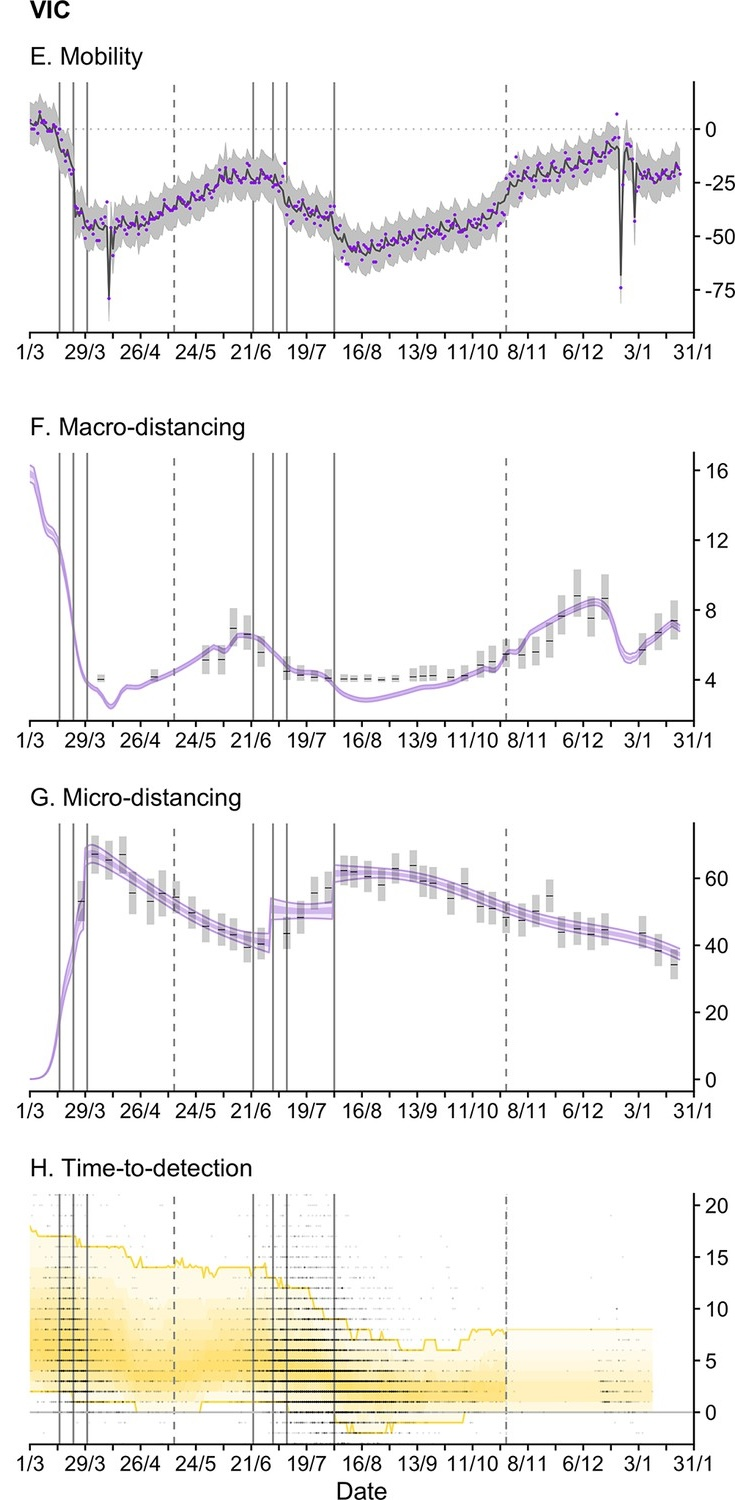
\includegraphics{images/lax_78089_elife-78089-fig3-v2.tif.jpg}
\end{column}

\begin{column}{0.3\textwidth}
\begin{itemize}
\tightlist
\item
  Staying safe \pause
\item
  Weekly Situational Assessment reports \pause
\item
  Transmission potential \pause
\item
  Dan Murphy's opening hours
\end{itemize}
\end{column}
\end{columns}

Golding et al.~2023. eLife
\end{frame}

\begin{frame}{Naturally you recall that}
\phantomsection\label{naturally-you-recall-that}
\begin{columns}[T]
\begin{column}{0.4\textwidth}
\begin{itemize}
\tightlist
\item
  Transmission potential makes boring times of low or no transmission
  more fun
\end{itemize}
\end{column}

\begin{column}{0.7\textwidth}
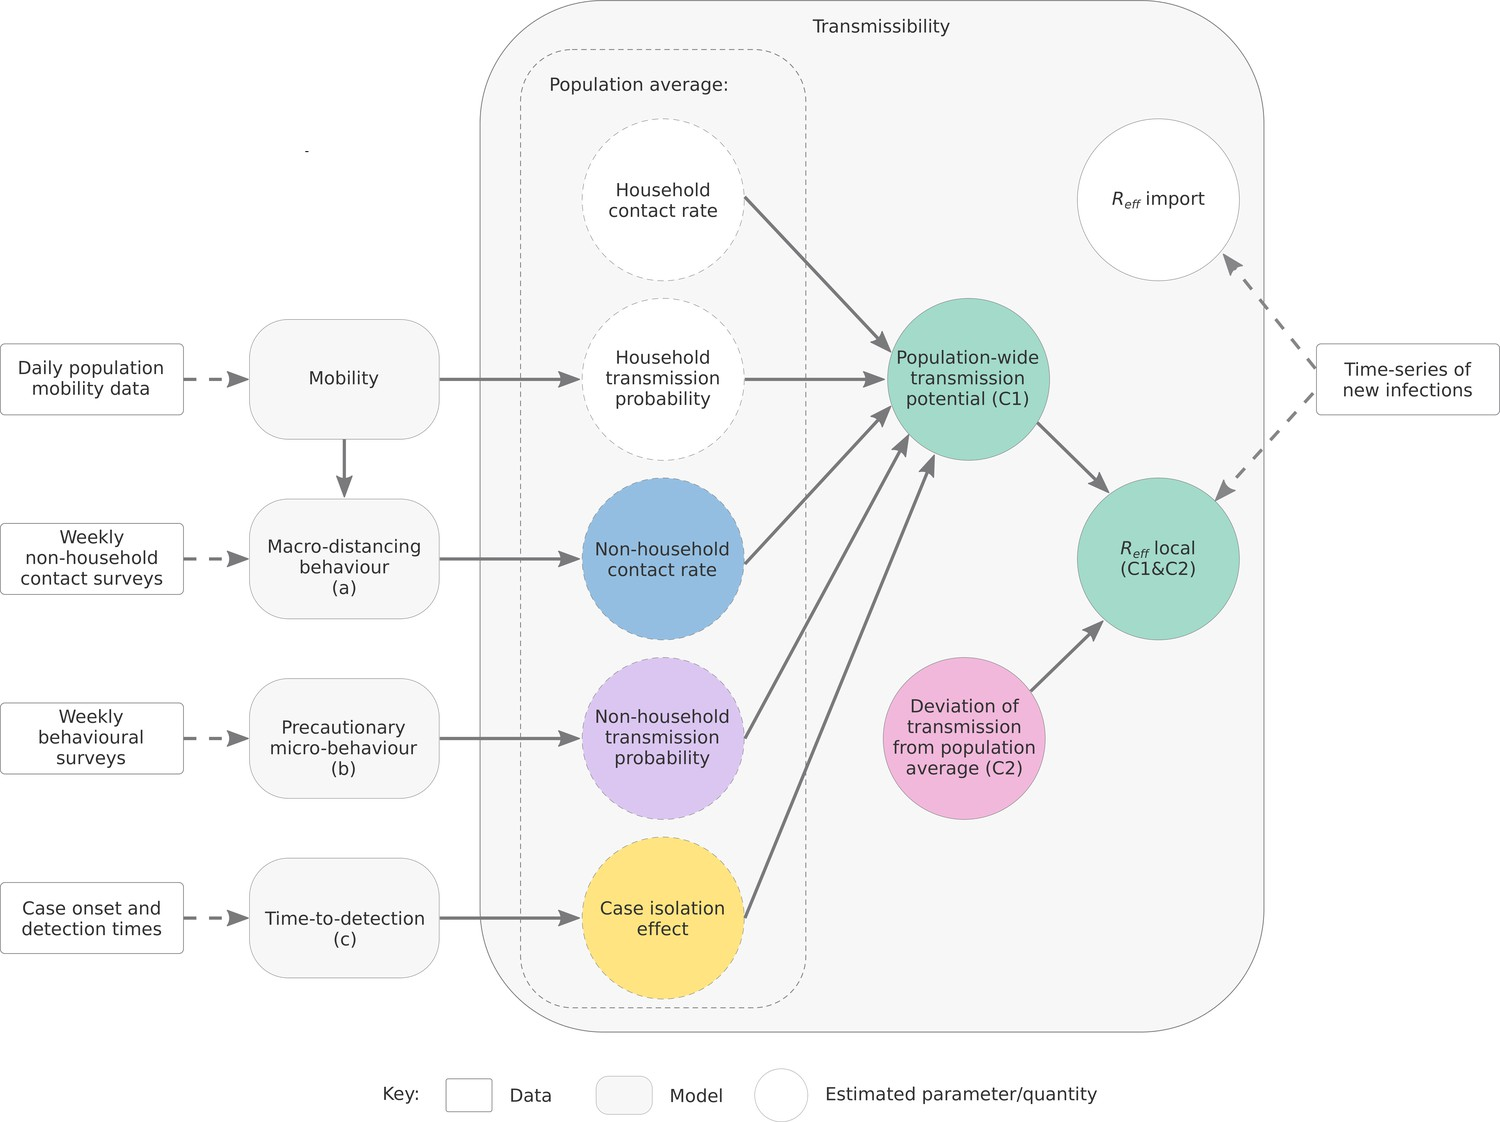
\includegraphics{images/tp_model_schema.jpg} Golding et al.~2023. eLife
\end{column}
\end{columns}
\end{frame}

\begin{frame}{Naturally you recall that}
\phantomsection\label{naturally-you-recall-that-1}
\begin{columns}[T]
\begin{column}{0.4\textwidth}
\begin{itemize}
\tightlist
\item
  Transmission potential makes boring times of low or no transmission
  more fun
\item
  TP is informed by behavioural data
\end{itemize}
\end{column}

\begin{column}{0.7\textwidth}
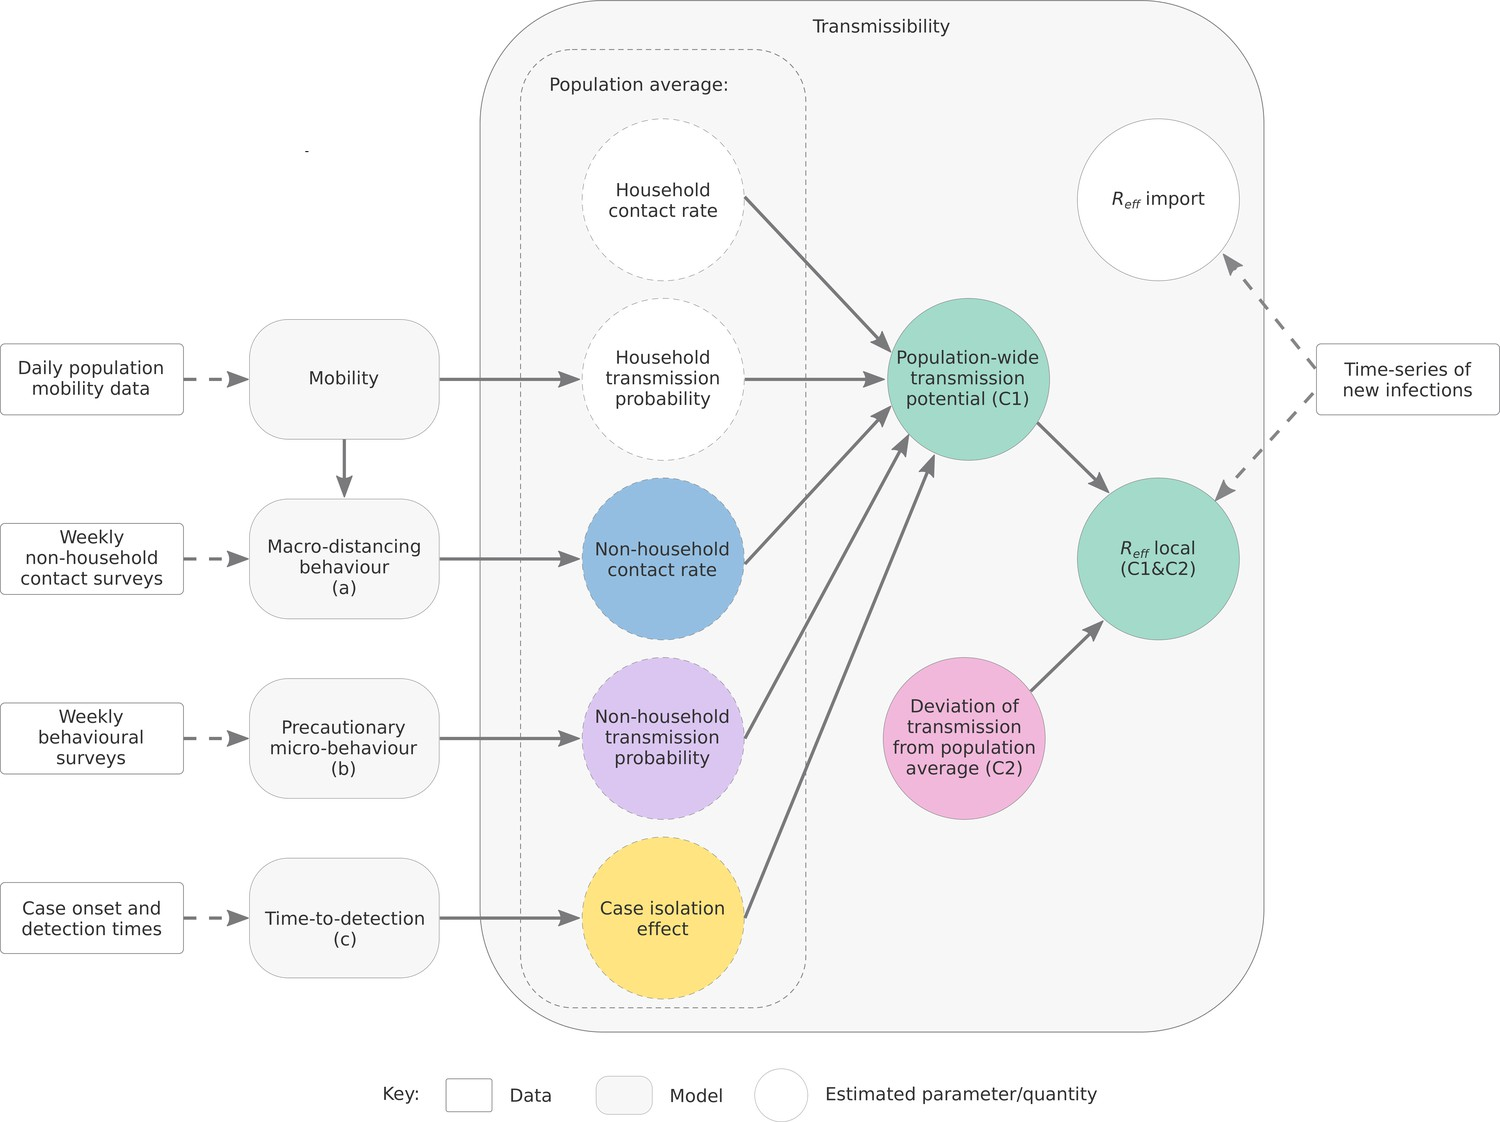
\includegraphics{images/tp_model_schema.jpg} Golding et al.~2023. eLife
\end{column}
\end{columns}
\end{frame}

\begin{frame}{Naturally you recall that}
\phantomsection\label{naturally-you-recall-that-2}
\begin{columns}[T]
\begin{column}{0.4\textwidth}
\begin{itemize}
\tightlist
\item
  Transmission potential makes boring times of low or no transmission
  more fun
\item
  TP is informed by behavioural data

  \begin{itemize}
  \tightlist
  \item
    mobility data
  \item
    questionnaire data
  \end{itemize}
\end{itemize}
\end{column}

\begin{column}{0.7\textwidth}
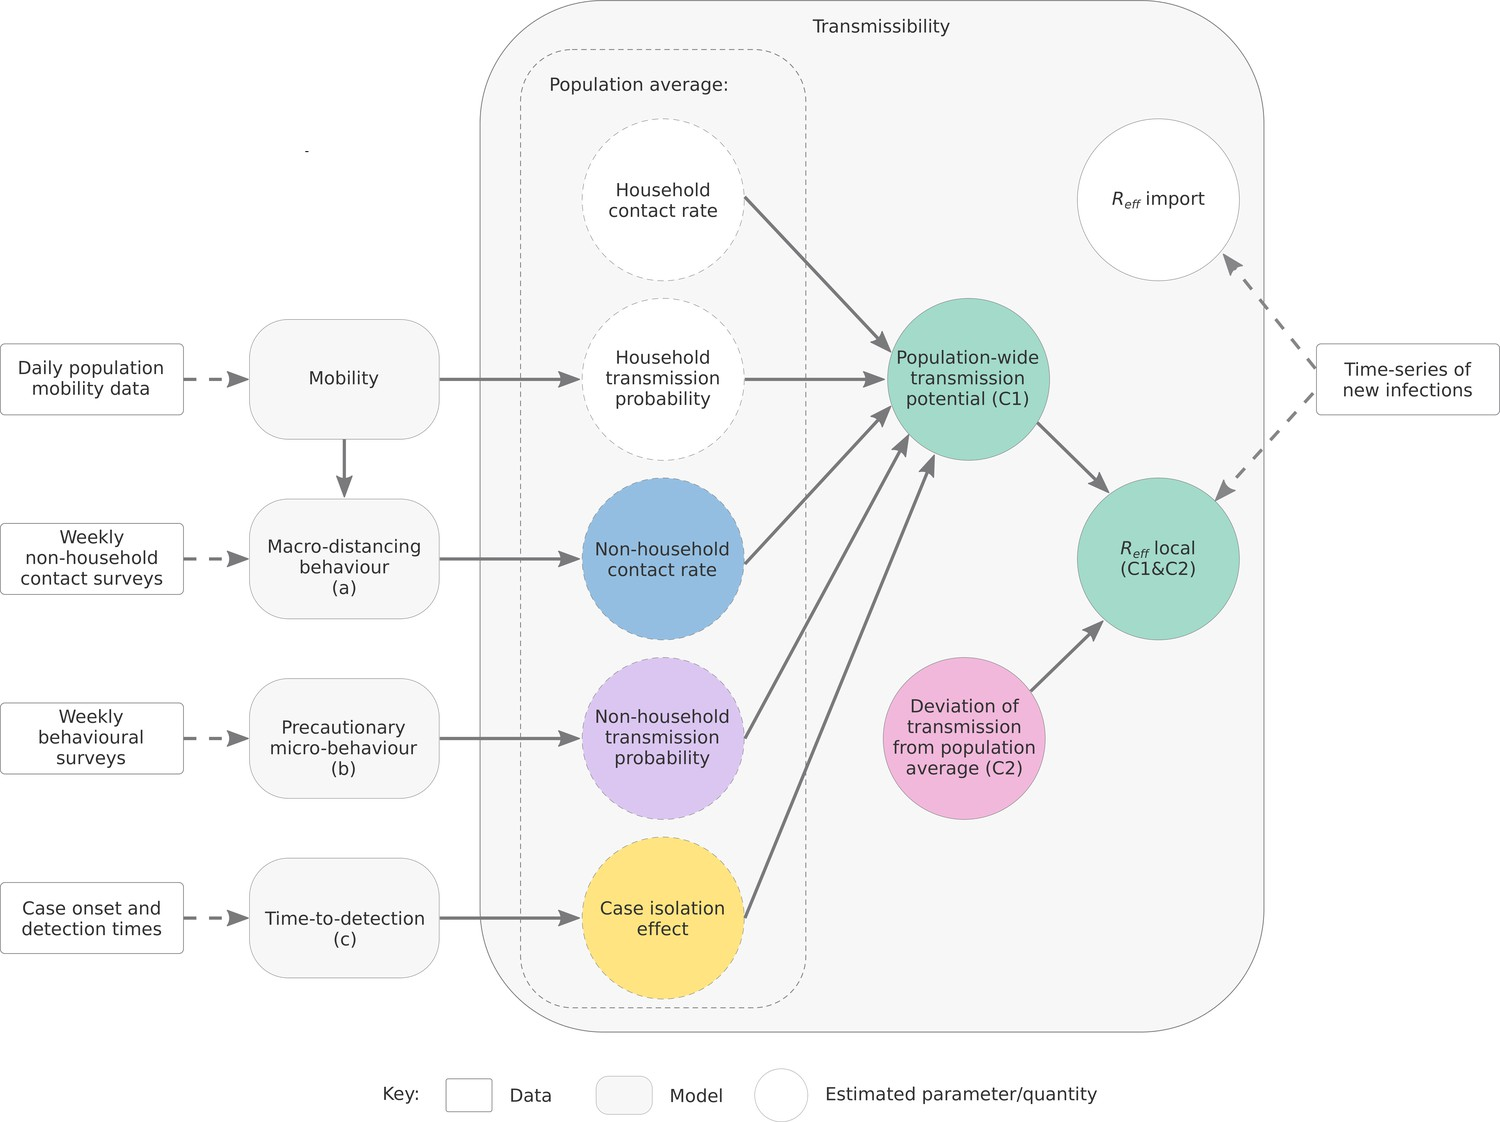
\includegraphics{images/tp_model_schema.jpg} Golding et al.~2023. eLife
\end{column}
\end{columns}
\end{frame}

\section{Mobility}\label{mobility}

\begin{frame}{We're all in it together}
\phantomsection\label{were-all-in-it-together}
\begin{columns}[T]
\begin{column}{0.4\textwidth}
Remember all the great data that Big Tech let us have?

\begin{itemize}
\tightlist
\item
  FaceBook!
\item
  CityMapper!
\item
  Apple!
\item
  Google!
\end{itemize}
\end{column}

\begin{column}{0.6\textwidth}
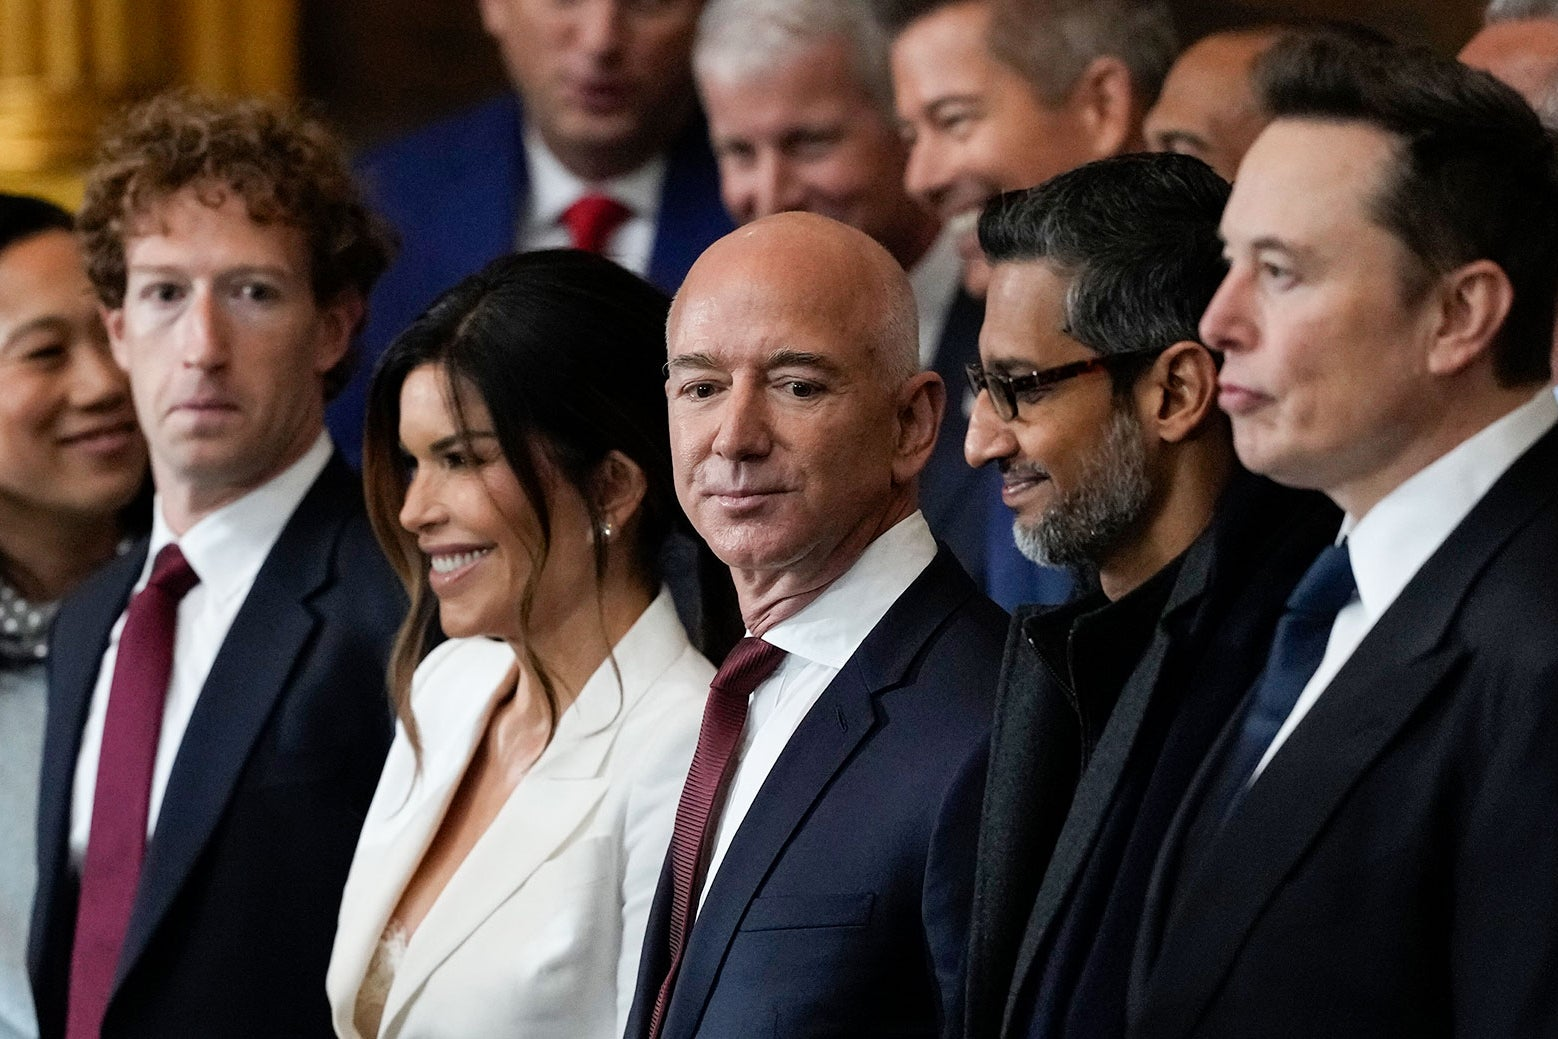
\includegraphics{images/tech_knobs.jpeg}
\end{column}
\end{columns}
\end{frame}

\begin{frame}{We're all in it together}
\phantomsection\label{were-all-in-it-together-1}
\begin{columns}[T]
\begin{column}{0.4\textwidth}
Remember all the great data that Big Tech let us have?

\begin{itemize}
\tightlist
\item
  \st{FaceBook!} RIP May 2020 ⚰️
\item
  CityMapper!
\item
  Apple!
\item
  Google!
\end{itemize}
\end{column}

\begin{column}{0.6\textwidth}
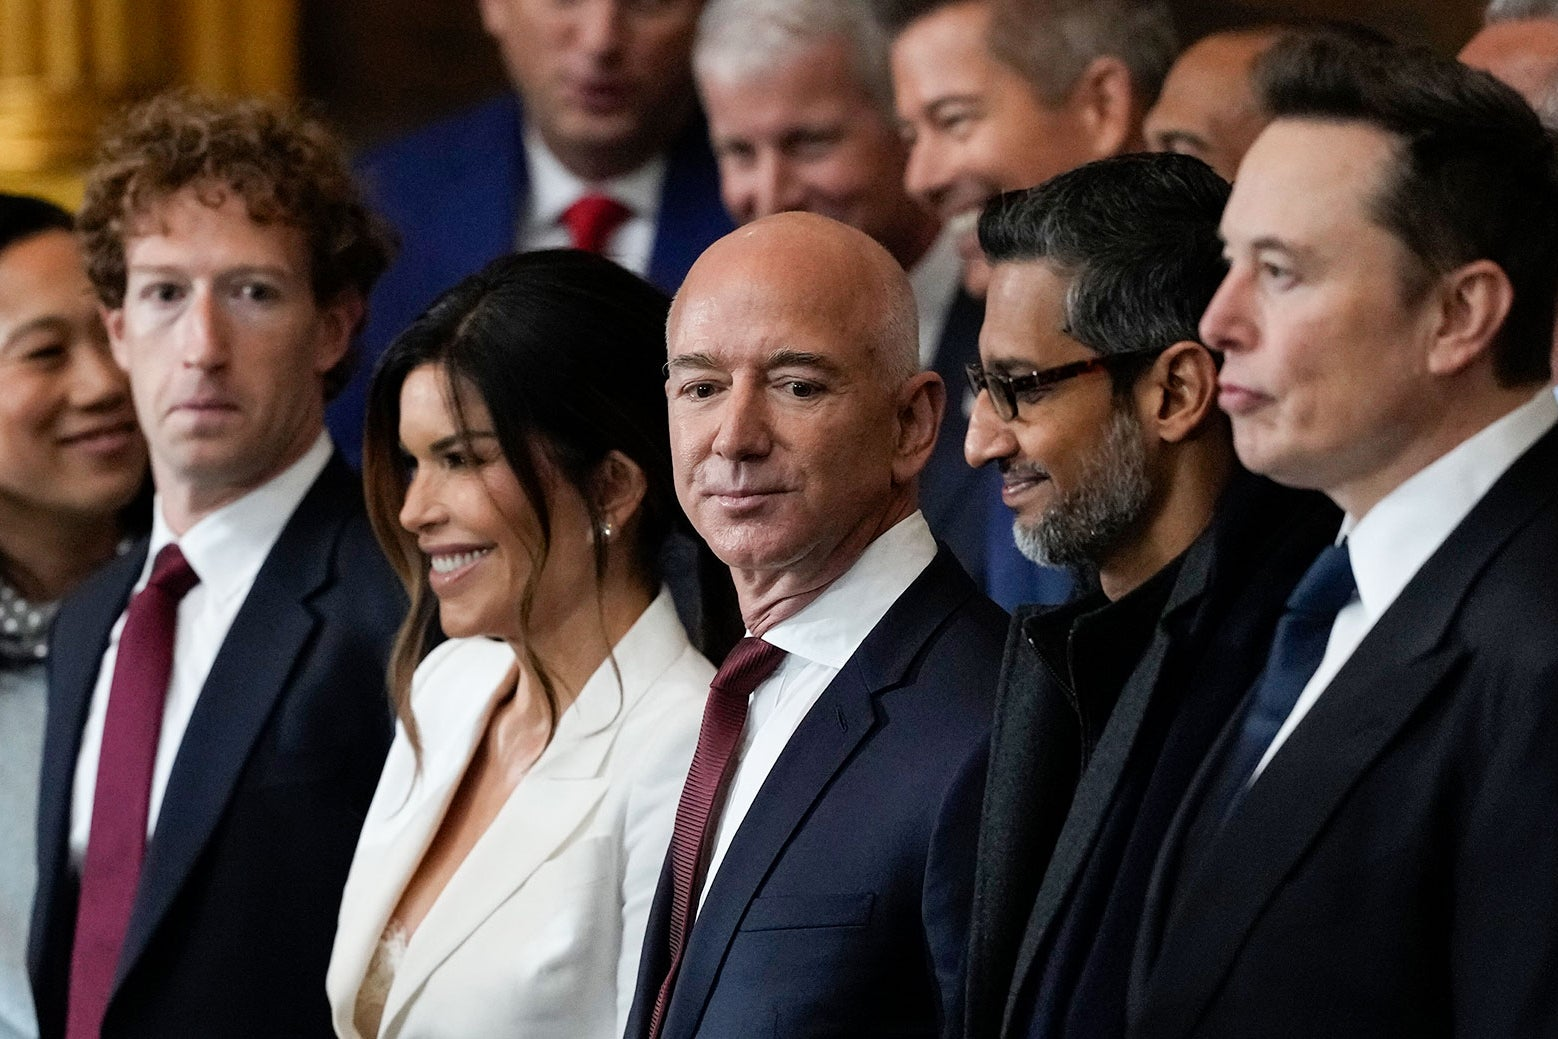
\includegraphics{images/tech_knobs.jpeg}
\end{column}
\end{columns}
\end{frame}

\begin{frame}{We're all in it together}
\phantomsection\label{were-all-in-it-together-2}
\begin{columns}[T]
\begin{column}{0.4\textwidth}
Remember all the great data that Big Tech let us have?

\begin{itemize}
\tightlist
\item
  \st{FaceBook!} RIP May 2020 ⚰️
\item
  \st{CityMapper!} RIP August 2021 ⚰️
\item
  \st{Apple!} RIP August 2021 2020 ⚰️
\item
  Google!
\end{itemize}
\end{column}

\begin{column}{0.6\textwidth}
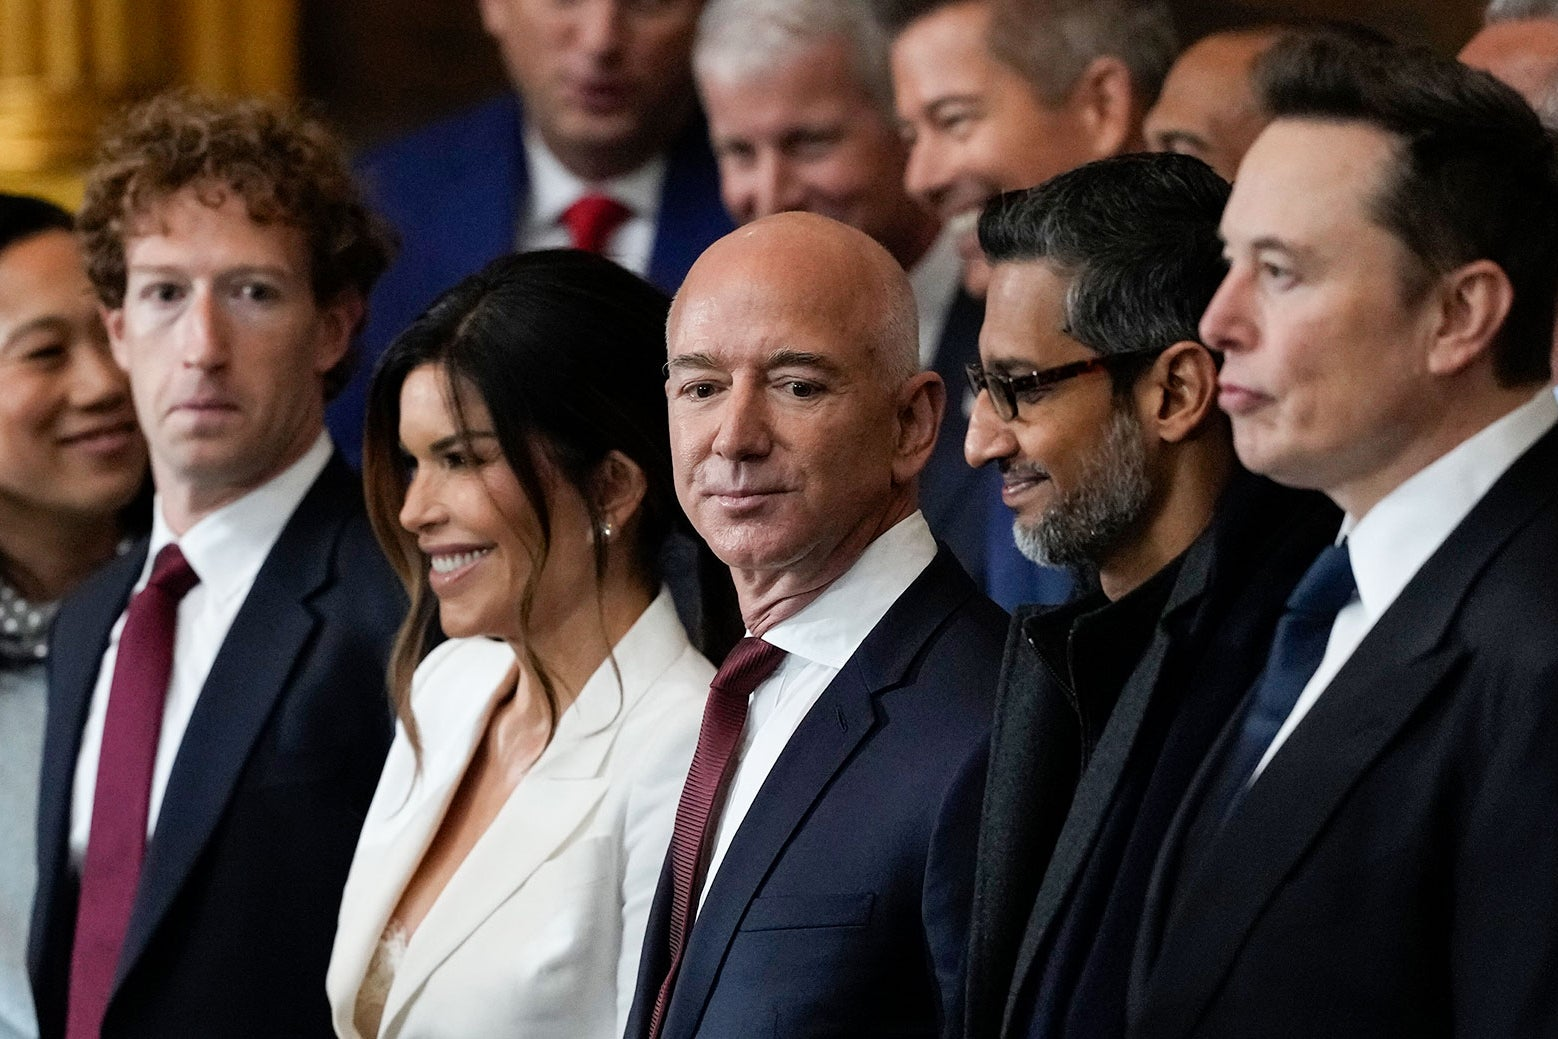
\includegraphics{images/tech_knobs.jpeg}
\end{column}
\end{columns}
\end{frame}

\begin{frame}{two col template}
\phantomsection\label{two-col-template}
\begin{columns}[T]
\begin{column}{0.48\textwidth}
\begin{itemize}
\tightlist
\item
  text
\item
  more
\end{itemize}
\end{column}

\begin{column}{0.48\textwidth}
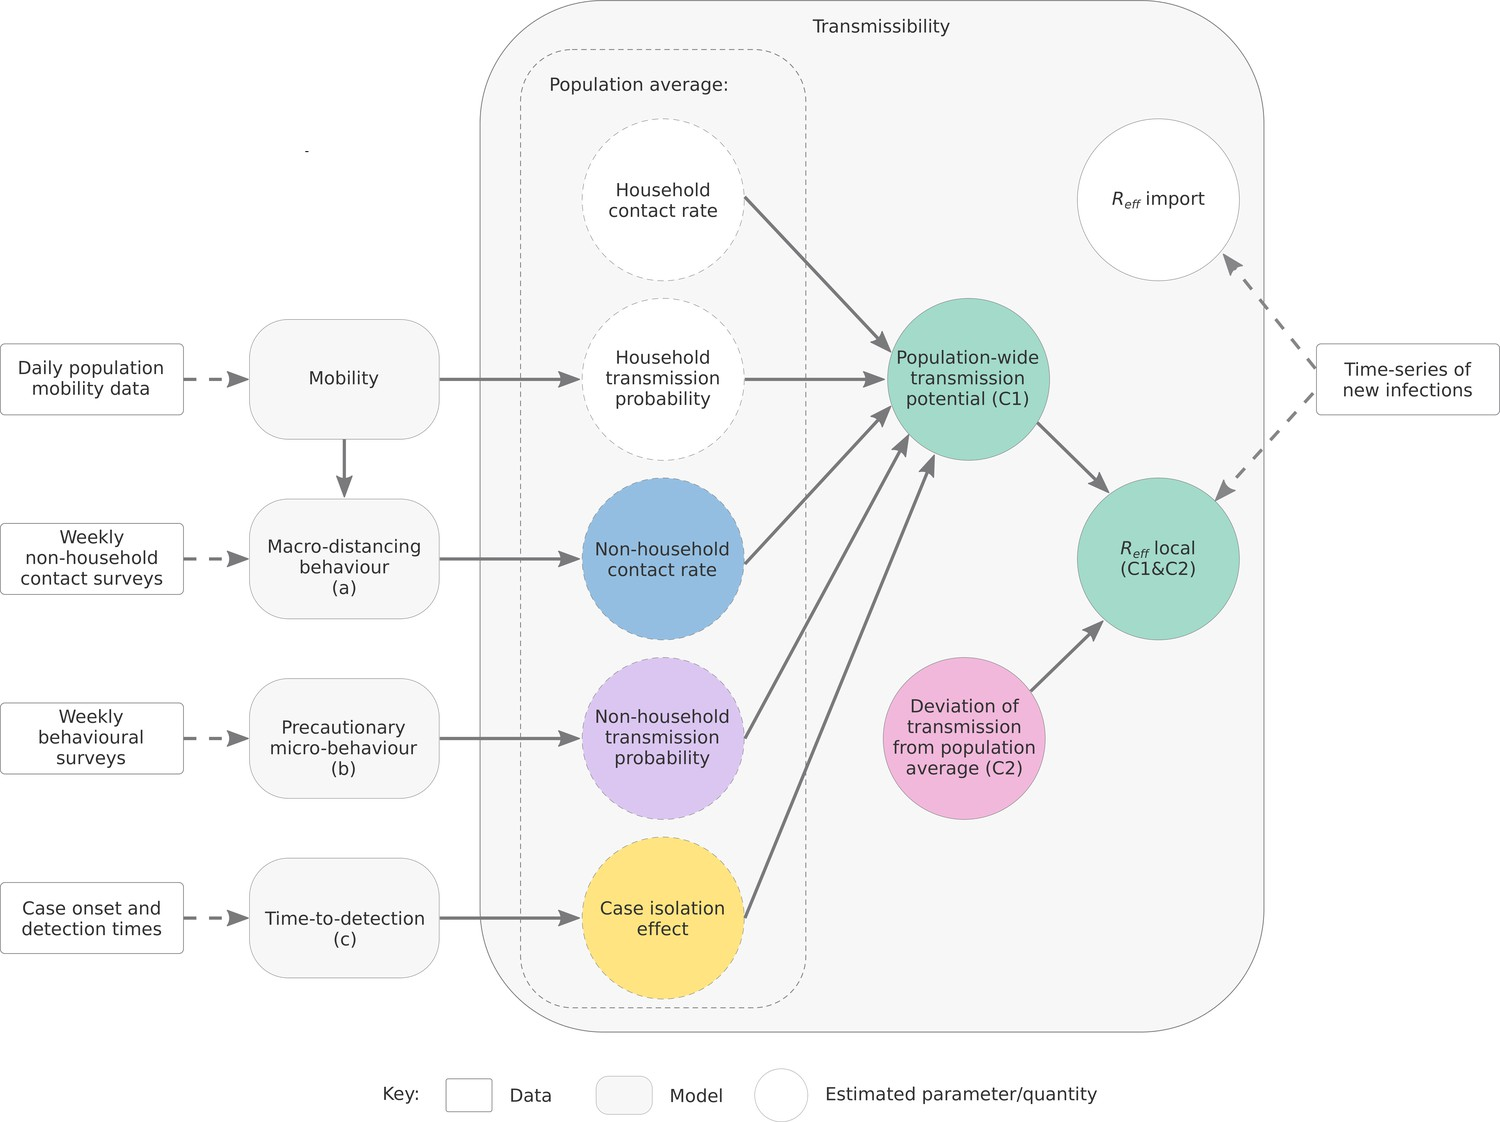
\includegraphics{images/tp_model_schema.jpg}
\end{column}
\end{columns}
\end{frame}




\end{document}
